\lecture{3}{Rotman §2.7}{Group Actions}

\section{Group Actions}

Groups of permutations led us to abstract groups. In this section we go back the other way:
every group can be realized as a group of permutations, and, more usefully, a group can be
studied by letting it \emph{act} on a set. The payoff includes a classification of the
groups of order at most \(7\), Cauchy's theorem, the structure of \(p\)-groups, and the
simplicity of the alternating groups \(A_n\) for \(n \geq 5\).

\subsection{What We Need from Homomorphisms and Quotient Groups}

This section uses some vocabulary from Rotman §2.5--§2.6. We collect it here.

\begin{recall}[Homomorphisms, normal subgroups, center]
	Let \(G\) and \(H\) be groups.
	\begin{itemize}
		\item A function \(f\colon G \to H\) is a \vocab{homomorphism} if
		      \(f(ab) = f(a)f(b)\) for all \(a, b \in G\). A bijective homomorphism is an
		      \vocab{isomorphism}; if one exists we write \(G \cong H\).
		\item The \vocab{kernel} of a homomorphism \(f\) is
		      \(\ker f = \{a \in G : f(a) = 1\}\), and its \vocab{image} is
		      \(\im f = \{f(a) : a \in G\}\).
		\item A subgroup \(K \leq G\) is \vocab{normal}, written \(K \trianglelefteq G\), if
		      \(gkg^{-1} \in K\) for all \(g \in G\) and \(k \in K\).
		\item The \vocab{center} of \(G\) is
		      \(Z(G) = \{z \in G : zg = gz \text{ for all } g \in G\}\).
	\end{itemize}
\end{recall}

\begin{proposition}[Facts from Rotman §2.5--§2.6]\label{prop:hom-facts}
	Let \(G\) be a group.
	\begin{enumerate}[(i)]
		\item If \(f\colon G \to H\) is a homomorphism, then \(f(1) = 1\),
		      \(f(a^{-1}) = f(a)^{-1}\), and \(\ker f \trianglelefteq G\). Moreover \(f\) is
		      injective if and only if \(\ker f = \{1\}\). If \(f\) is an isomorphism, then
		      \(a\) and \(f(a)\) have the same order for every \(a \in G\).
		\item Every subgroup of \(Z(G)\) is a normal subgroup of \(G\); in particular
		      \(Z(G) \trianglelefteq G\), and every subgroup of an abelian group is normal.
		\item \emph{(Quotient groups)} If \(K \trianglelefteq G\), then the family \(G/K\)
		      of all cosets of \(K\) is a group under \((aK)(bK) = abK\), with identity
		      \(K\); it has order \(\abs{G/K} = [G:K]\).
		\item \emph{(Correspondence theorem)} If \(K \trianglelefteq G\), then
		      \(S \mapsto S/K\) is a bijection from the subgroups \(S\) with
		      \(K \leq S \leq G\) onto the subgroups of \(G/K\); moreover
		      \(S \trianglelefteq G\) if and only if \(S/K \trianglelefteq G/K\).
		\item Two cyclic groups of the same order are isomorphic. Together with
		      \autoref{cor:prime-order-cyclic}: every group of prime order \(p\) is
		      isomorphic to \(\mathbb Z_p\).
		\item \emph{(Rotman, Proposition 2.122)} If \(G\) is a finite \emph{abelian} group,
		      then \(G\) has a subgroup of order \(d\) for every divisor \(d\) of \(\abs{G}\).
		      In particular, if a prime \(p\) divides \(\abs{G}\), then \(G\) contains an
		      element of order \(p\).
	\end{enumerate}
\end{proposition}

The next few facts appear as exercises in Rotman; we shall use them repeatedly, so we
prove them here.

\begin{lemma}[Rotman, Exercise 2.56]\label{lem:SX-iso}
	If \(f\colon X \to Y\) is a bijection, then
	\(\varphi\colon S_X \to S_Y\), \(\varphi(\sigma) = f\sigma f^{-1}\), is an isomorphism.
	In particular, if \(\abs{X} = n\), then \(S_X \cong S_n\). If \(X\) and \(Y\) are
	finite, then \(\varphi\) carries each cycle \((x_1\ \dots\ x_r)\) to the cycle
	\((f(x_1)\ \dots\ f(x_r))\), so it preserves cycle structure and parity.
\end{lemma}

\begin{proof}
	\(f\sigma f^{-1}\) is a composite of bijections \(Y \to X \to X \to Y\), so it lies in
	\(S_Y\). We have
	\(\varphi(\sigma)\varphi(\tau) = f\sigma f^{-1} f\tau f^{-1} = f\sigma\tau f^{-1}
	= \varphi(\sigma\tau)\), and \(\pi \mapsto f^{-1}\pi f\) is an inverse of
	\(\varphi\). The statement about cycles is checked exactly as in
	\autoref{lem:conj-action}: if \(\sigma(x) = x'\), then
	\(f\sigma f^{-1}(f(x)) = f(x')\).
\end{proof}

\begin{lemma}[Rotman, Exercise 2.38]\label{lem:exponent-two}
	If \(x^2 = 1\) for every \(x\) in a group \(G\), then \(G\) is abelian.
\end{lemma}

\begin{proof}
	The hypothesis says \(x = x^{-1}\) for all \(x\). Hence, for \(x, y \in G\),
	\(xy = (xy)^{-1} = y^{-1}x^{-1} = yx\).
\end{proof}

\begin{lemma}[Rotman, Exercise 2.40]\label{lem:even-order}
	A finite group \(G\) of even order contains an element of order \(2\).
\end{lemma}

\begin{proof}
	Pair each \(x \in G\) with \(x^{-1}\). The elements with \(x \neq x^{-1}\) fall into
	pairs \(\{x, x^{-1}\}\), so there is an even number of them. Hence the set
	\(\{x \in G : x = x^{-1}\}\) has even size too. It contains \(1\), so it contains some
	\(x \neq 1\), and such an \(x\) satisfies \(x^2 = 1\), that is, \(x\) has order \(2\).
\end{proof}

\begin{lemma}[Rotman, Exercise 2.87]\label{lem:center-cyclic}
	If \(G/Z(G)\) is cyclic, then \(G\) is abelian.
\end{lemma}

\begin{proof}
	Write \(Z = Z(G)\) and \(G/Z = \langle aZ\rangle\). Every coset has the form
	\((aZ)^i = a^iZ\), so every \(g \in G\) can be written \(g = a^i z\) with
	\(z \in Z\). If also \(h = a^j z'\), then, since \(z, z'\) commute with everything,
	\[
		gh = a^i z a^j z' = a^{i+j}zz' = a^j z' a^i z = hg. \qedhere
	\]
\end{proof}

\begin{lemma}[Rotman, Proposition 2.127]\label{lem:coprime-orders}
	Let \(a, b\) be commuting elements of a group, of orders \(m\) and \(n\). If
	\(\gcd(m,n) = 1\), then \(ab\) has order \(mn\).
\end{lemma}

\begin{proof}
	Since \(ab = ba\), we have \((ab)^r = a^rb^r\) for all \(r\), so
	\((ab)^{mn} = (a^m)^n(b^n)^m = 1\). Conversely suppose \((ab)^k = 1\). Then
	\(a^k = b^{-k}\) lies in \(\langle a\rangle \cap \langle b\rangle\). The order of
	this subgroup divides both \(m = \abs{\langle a\rangle}\) and
	\(n = \abs{\langle b\rangle}\) by Lagrange's theorem, hence equals \(1\); so
	\(a^k = 1 = b^k\), and \autoref{lem:order-divides} gives \(m \mid k\) and \(n \mid k\).
	Write \(k = mq\) and choose \(x, y\) with \(mx + ny = 1\)
	(\autoref{cor:bezout-criterion}); then \(q = mqx + nqy = kx + nqy\) is divisible by
	\(n\), so \(mn \mid k\). Therefore the order of \(ab\) is \(mn\).
\end{proof}

\subsection{Cayley's Theorem}

The next result, due to A.~Cayley (1821--1895), shows that abstract groups are not so far
removed from permutations.

\begin{theorem}[Cayley]\label{thm:cayley}
	Every group \(G\) is (isomorphic to) a subgroup of the symmetric group \(S_G\). In
	particular, if \(\abs{G} = n\), then \(G\) is isomorphic to a subgroup of \(S_n\).
\end{theorem}

\begin{proof}
	For each \(a \in G\), define the \vocab{translation} \(\tau_a\colon G \to G\) by
	\(\tau_a(x) = ax\). (If \(a \neq 1\), then \(\tau_a\) is \emph{not} a homomorphism,
	since \(\tau_a(1) = a \neq 1\).) For \(a, b \in G\) and every \(x \in G\),
	\[
		(\tau_a \circ \tau_b)(x) = \tau_a(bx) = a(bx) = (ab)x = \tau_{ab}(x),
	\]
	by associativity, so that
	\[
		\tau_a\tau_b = \tau_{ab}.
	\]
	It follows that each \(\tau_a\) is a bijection, with inverse \(\tau_{a^{-1}}\):
	\(\tau_a\tau_{a^{-1}} = \tau_1 = 1_G = \tau_{a^{-1}}\tau_a\). Thus
	\(\tau_a \in S_G\).

	Define \(\varphi\colon G \to S_G\) by \(\varphi(a) = \tau_a\). The displayed equation
	says \(\varphi(a)\varphi(b) = \varphi(ab)\), so \(\varphi\) is a homomorphism. It is
	injective: if \(\varphi(a) = \varphi(b)\), then \(\tau_a(x) = \tau_b(x)\) for all
	\(x\), and \(x = 1\) gives \(a = b\). Hence \(G \cong \im\varphi \leq S_G\).

	The last statement follows from \autoref{lem:SX-iso}: if \(\abs{G} = n\), then
	\(S_G \cong S_n\).
\end{proof}

\begin{remark}
	In the proof, the permutation \(\tau_a\) is just the row labelled \(a\) of the
	multiplication table of \(G\).
\end{remark}

\begin{eg}[Cayley's theorem for \(\mathbb Z_3\)]
	Take \(G = \mathbb Z_3 = \{[0],[1],[2]\}\) (written additively, so
	\(\tau_a(x) = a + x\)). Labelling \([0],[1],[2]\) as \(1,2,3\), we get
	\(\tau_{[0]} = (1)\), \(\tau_{[1]} = (1\ 2\ 3)\), \(\tau_{[2]} = (1\ 3\ 2)\). Thus
	\(\mathbb Z_3\) is isomorphic to the subgroup \(A_3 = \langle(1\ 2\ 3)\rangle\) of
	\(S_3\).
\end{eg}

To tell the truth, Cayley's theorem by itself is only mildly interesting. However, the
identical proof works in a larger setting that is more useful. Even when \(H\) is not a
normal subgroup, we still write \(G/H\) for the family of all (left) cosets of \(H\) in
\(G\).

\begin{theorem}[Representation on cosets]\label{thm:rep-on-cosets}
	Let \(G\) be a group and let \(H\) be a subgroup of \(G\) having finite index \(n\).
	Then there is a homomorphism \(\varphi\colon G \to S_n\) with \(\ker\varphi \leq H\).
\end{theorem}

\begin{proof}
	For each \(a \in G\) define \(\tau_a\colon G/H \to G/H\) by \(\tau_a(xH) = axH\); this
	is well defined, because \(xH = yH\) means \(y^{-1}x \in H\), and then
	\((ay)^{-1}(ax) = y^{-1}x \in H\), so \(axH = ayH\). For \(a, b \in G\),
	\[
		(\tau_a \circ \tau_b)(xH) = \tau_a(bxH) = a(bx)H = (ab)xH = \tau_{ab}(xH),
	\]
	so again \(\tau_a\tau_b = \tau_{ab}\). As before each \(\tau_a\) is a bijection with
	inverse \(\tau_{a^{-1}}\), for \(\tau_a\tau_{a^{-1}} = \tau_1 = 1_{G/H}
	= \tau_{a^{-1}}\tau_a\); so \(\tau_a \in S_{G/H}\), and
	\(\varphi\colon G \to S_{G/H}\), \(\varphi(a) = \tau_a\), is a homomorphism.

	If \(a \in \ker\varphi\), then \(\tau_a = 1_{G/H}\), so \(axH = xH\) for all
	\(x \in G\); taking \(x = 1\) gives \(aH = H\), and hence \(a \in H\) by
	\autoref{lem:coset-basics}(i). Thus \(\ker\varphi \leq H\).

	Finally \(\abs{G/H} = n\), so \(S_{G/H} \cong S_n\) by \autoref{lem:SX-iso}; composing
	\(\varphi\) with this isomorphism does not change the kernel.
\end{proof}

When \(H = \{1\}\), this is Cayley's theorem.

\subsection{Groups of Small Order}

We now classify all groups of order at most \(7\). By
\autoref{prop:hom-facts}(v), every group of prime order \(p\) is isomorphic to
\(\mathbb Z_p\), so up to isomorphism there is just one group of order \(p\). Of the
orders \(2, \dots, 7\), four are primes (\(2, 3, 5, 7\)), so we need only look at orders
\(4\) and \(6\).

\begin{proposition}\label{prop:order-4}
	Every group \(G\) of order \(4\) is isomorphic to either \(\mathbb Z_4\) or the
	four-group \(\mathbf V\). Moreover, \(\mathbb Z_4\) and \(\mathbf V\) are not
	isomorphic.
\end{proposition}

\begin{proof}
	By Lagrange's theorem, every element of \(G\) other than \(1\) has order \(2\) or
	\(4\). If there is an element of order \(4\), then \(G\) is cyclic, and
	\(G \cong \mathbb Z_4\). Otherwise \(x^2 = 1\) for all \(x \in G\), so \(G\) is abelian
	by \autoref{lem:exponent-two}.

	Choose distinct \(x, y \in G\), neither equal to \(1\). Then
	\(xy \notin \{1, x, y\}\): \(xy = 1\) would give \(y = x^{-1} = x\), \(xy = x\) would
	give \(y = 1\), and \(xy = y\) would give \(x = 1\). Hence
	\[
		G = \{1, x, y, xy\}.
	\]
	The product of any two distinct elements of order \(2\) is the third one (e.g.\
	\(x \cdot xy = x^2y = y\)), and exactly the same is true in \(\mathbf V\). Therefore the
	bijection \(f\colon G \to \mathbf V\) defined by
	\[
		f(1) = (1), \quad f(x) = (1\ 2)(3\ 4), \quad f(y) = (1\ 3)(2\ 4), \quad
		f(xy) = (1\ 4)(2\ 3)
	\]
	is an isomorphism.

	Finally, \(\mathbb Z_4 \not\cong \mathbf V\): an isomorphism preserves orders of
	elements (\autoref{prop:hom-facts}(i)), but \(\mathbb Z_4\) has an element of order
	\(4\), while every element of \(\mathbf V\) has order at most \(2\).
\end{proof}

\begin{proposition}\label{prop:order-6}
	If \(G\) is a group of order \(6\), then \(G\) is isomorphic to either \(\mathbb Z_6\)
	or \(S_3\). Moreover, \(\mathbb Z_6\) and \(S_3\) are not isomorphic.
\end{proposition}

\begin{proof}
	By Lagrange's theorem, the only possible orders of nonidentity elements are \(2\),
	\(3\), and \(6\). Of course \(G \cong \mathbb Z_6\) if \(G\) has an element of order
	\(6\). By \autoref{lem:even-order}, \(G\) contains an element \(t\) of order \(2\); let
	\(T = \langle t\rangle = \{1, t\}\).

	Since \([G:T] = 3\), the representation on the cosets of \(T\)
	(\autoref{thm:rep-on-cosets}) is a homomorphism \(\rho\colon G \to S_{G/T} \cong S_3\)
	with \(\ker\rho \leq T\). Thus \(\ker\rho = \{1\}\) or \(\ker\rho = T\).

	\emph{Case \(\ker\rho = \{1\}\).} Then \(\rho\) is injective, and hence bijective, since
	\(\abs{G} = 6 = \abs{S_3}\). So \(G \cong S_3\).

	\emph{Case \(\ker\rho = T\).} Then \(T \trianglelefteq G\), and the quotient group
	\(G/T\) is defined. It has order \(3\), so it is cyclic: there is \(a \in G\) with
	\(G/T = \{T, aT, a^2T\}\). Moreover \(\rho_t\) is the permutation
	\[
		\rho_t = \begin{pmatrix} T & aT & a^2T \\ tT & taT & ta^2T \end{pmatrix}.
	\]
	Since \(t \in T = \ker\rho\), \(\rho_t\) is the identity; in particular
	\(aT = \rho_t(aT) = taT\), so that \(a^{-1}ta \in T = \{1, t\}\) by
	\autoref{lem:coset-basics}(i). But \(a^{-1}ta \neq 1\) because \(t \neq 1\); hence
	\(a^{-1}ta = t\), that is, \(ta = at\).

	Now \(aT \neq T\) and \(a^2T \neq T\), so \(a \neq 1\) and \(a^2 \neq 1\); thus \(a\)
	has order \(3\) or \(6\). In either case \(G\) has an element of order \(6\): if \(a\)
	has order \(3\), then \(at\) has order \(6\) by \autoref{lem:coprime-orders}.
	Therefore \(G\) is cyclic of order \(6\), and \(G \cong \mathbb Z_6\).

	Finally, \(\mathbb Z_6 \not\cong S_3\), for one is abelian and the other is not.
\end{proof}

\begin{remark}
	Cayley stated this proposition in 1854. In 1878, however, he wrote that for \(n = 6\)
	``there are three groups'': the cyclic one, and two more generated by \(\alpha, \beta\)
	with \(\alpha^2 = 1\), \(\beta^3 = 1\), one with \(\alpha\beta = \beta\alpha\) and one
	with \(\alpha\beta = \beta^2\alpha\). His list is \(\mathbb Z_6\),
	\(\mathbb Z_2 \times \mathbb Z_3\), and \(S_3\); but
	\(\mathbb Z_2 \times \mathbb Z_3 \cong \mathbb Z_6\). Even Homer nods.
\end{remark}

Classifying groups of order \(8\) is more difficult, for we have not yet developed enough
theory. It turns out that there are exactly \(5\) nonisomorphic groups of order \(8\):
three are abelian,
\[
	\mathbb Z_8, \qquad \mathbb Z_4 \times \mathbb Z_2, \qquad
	\mathbb Z_2 \times \mathbb Z_2 \times \mathbb Z_2,
\]
and two are nonabelian: the dihedral group \(D_8\) and the quaternions \(\mathbf Q\).

\begin{table}[H]
	\centering
	\begin{tabular}{rr}
		\toprule
		Order of group & Number of groups \\
		\midrule
		\(2\)    & \(1\)              \\
		\(4\)    & \(2\)              \\
		\(8\)    & \(5\)              \\
		\(16\)   & \(14\)             \\
		\(32\)   & \(51\)             \\
		\(64\)   & \(267\)            \\
		\(128\)  & \(2{,}328\)        \\
		\(256\)  & \(56{,}092\)       \\
		\(512\)  & \(10{,}494{,}213\) \\
		\(1024\) & \(49{,}487{,}365{,}422\) \\
		\bottomrule
	\end{tabular}
	\caption{The number of nonisomorphic groups of order \(2^k\).}
	\label{tab:groups-of-order-2k}
\end{table}

One can continue this discussion for larger orders, but things soon get out of hand, as
\autoref{tab:groups-of-order-2k} shows. A.~McIver and P.~M.~Neumann proved that the number
of nonisomorphic groups of order \(n\) is at most \(n^{\mu^2+\mu+2}\), where \(\mu\) is
the largest exponent occurring in the prime factorization of \(n\). Obviously, making a
telephone directory of groups is not the way to study them.

\subsection{Actions, Orbits, and Stabilizers}

Groups arose by abstracting the fundamental properties enjoyed by permutations. But there
is an important feature of permutations that the axioms do not mention: permutations are
\emph{functions}. We shall see that there are interesting consequences when this feature
is restored.

\begin{notation}
	A function of two variables \(\alpha\colon X \times Y \to Z\) can be regarded as a
	one-parameter family of functions of one variable: each \(x \in X\) gives a function
	\(\alpha_x\colon Y \to Z\), namely \(\alpha_x(y) = \alpha(x,y)\).
\end{notation}

\begin{definition}[Group action]\label{def:action}
	If \(X\) is a set and \(G\) is a group, then \(G\) \vocab{acts on} \(X\) if there is a
	function \(\alpha\colon G \times X \to X\), called an \vocab{action}, such that
	\begin{enumerate}[(i)]
		\item \(\alpha_g \circ \alpha_h = \alpha_{gh}\) for all \(g, h \in G\);
		\item \(\alpha_1 = 1_X\), the identity function.
	\end{enumerate}
	If \(G\) acts on \(X\), one often calls \(X\) a \vocab{\(G\)-set}.
\end{definition}

\begin{notation}
	If \(G\) acts on \(X\), we usually write \(gx\) instead of \(\alpha_g(x)\). In this
	notation, axiom (i) reads \(g(hx) = (gh)x\), and axiom (ii) reads \(1x = x\).
\end{notation}

Of course, every subgroup \(G \leq S_X\) acts on \(X\) by evaluation,
\(\alpha_g(x) = g(x)\). More generally, actions of a group \(G\) on a set \(X\) are the
same thing as homomorphisms \(G \to S_X\).

\begin{proposition}\label{prop:action-hom}
	If \(\alpha\colon G \times X \to X\) is an action of a group \(G\) on a set \(X\), then
	\(g \mapsto \alpha_g\) defines a homomorphism \(G \to S_X\). Conversely, if
	\(B\colon G \to S_X\) is a homomorphism, then \(\beta\colon G \times X \to X\), defined
	by \(\beta(g,x) = B(g)(x)\), is an action.
\end{proposition}

\begin{proof}
	Let \(\alpha\) be an action. Each \(\alpha_g\) is a permutation of \(X\), with inverse
	\(\alpha_{g^{-1}}\), because
	\(\alpha_g\alpha_{g^{-1}} = \alpha_{gg^{-1}} = \alpha_1 = 1_X\) and likewise
	\(\alpha_{g^{-1}}\alpha_g = 1_X\). Hence \(A\colon G \to S_X\), \(A(g) = \alpha_g\), is
	a function with the stated target, and axiom (i) says precisely that it is a
	homomorphism:
	\[
		A(gh) = \alpha_{gh} = \alpha_g \circ \alpha_h = A(g) \circ A(h).
	\]

	Conversely, let \(B\colon G \to S_X\) be a homomorphism and
	\(\beta(g,x) = B(g)(x)\), so that \(\beta_g = B(g)\). Axiom (i) says
	\(B(g) \circ B(h) = B(gh)\), which holds because \(B\) is a homomorphism; axiom (ii),
	\(B(1) = 1_X\), holds because every homomorphism takes the identity to the identity
	(\autoref{prop:hom-facts}(i)).
\end{proof}

Cayley's theorem says that a group \(G\) acts on itself by (left) translation, and its
generalization \autoref{thm:rep-on-cosets} says that \(G\) also acts on the family
\(G/H\) of cosets of a subgroup \(H\) by (left) translation.

\begin{eg}[Conjugation]\label{eg:conjugation-action}
	A group \(G\) acts on itself by \vocab{conjugation}: for each \(g \in G\), define
	\(\alpha_g\colon G \to G\) by
	\[
		\alpha_g(x) = gxg^{-1}.
	\]
	To verify axiom (i), note that for each \(x \in G\),
	\begin{align*}
		(\alpha_g \circ \alpha_h)(x)
		 & = \alpha_g(hxh^{-1})
		= g(hxh^{-1})g^{-1}
		= (gh)x(gh)^{-1}
		= \alpha_{gh}(x).
	\end{align*}
	Therefore \(\alpha_g \circ \alpha_h = \alpha_{gh}\). For axiom (ii),
	\(\alpha_1(x) = 1x1^{-1} = x\) for each \(x\), so \(\alpha_1 = 1_G\).
\end{eg}

The following two definitions are fundamental.

\begin{definition}[Orbit, stabilizer]\label{def:orbit-stabilizer}
	Let \(G\) act on \(X\) and let \(x \in X\). The \vocab{orbit} of \(x\) is the subset
	\[
		\mathcal O(x) = \{gx : g \in G\} \subseteq X,
	\]
	and the \vocab{stabilizer} of \(x\) is
	\[
		G_x = \{g \in G : gx = x\}.
	\]
	We say \(G\) acts \vocab{transitively} on \(X\) if there is some \(x \in X\) with
	\(\mathcal O(x) = X\).
\end{definition}

\begin{lemma}\label{lem:stabilizer-subgroup}
	The stabilizer \(G_x\) of a point \(x \in X\) is a subgroup of \(G\).
\end{lemma}

\begin{proof}
	\(1 \in G_x\) since \(1x = x\). If \(g, h \in G_x\), then \((gh)x = g(hx) = gx = x\),
	so \(gh \in G_x\); and \(g^{-1}x = g^{-1}(gx) = (g^{-1}g)x = 1x = x\), so
	\(g^{-1} \in G_x\).
\end{proof}

Let us find orbits and stabilizers in the examples above.

\begin{eg}[Translations]\label{eg:translation-orbits}
	\begin{enumerate}[(i)]
		\item Let \(G\) act on itself by translation, \(\tau_a\colon x \mapsto ax\). If
		      \(x \in G\), then \(\mathcal O(x) = G\), for if \(g \in G\), then
		      \(g = (gx^{-1})x\). The stabilizer \(G_x\) is \(\{1\}\), for if
		      \(x = \tau_a(x) = ax\), then \(a = 1\). So \(G\) acts transitively on itself.
		\item Let \(G\) act on \(G/H\) by translation, \(\tau_a\colon xH \mapsto axH\).
		      Then \(\mathcal O(xH) = G/H\), for if \(g \in G\) and \(a = gx^{-1}\), then
		      \(\tau_a\colon xH \mapsto gH\). Thus \(G\) acts transitively on \(G/H\). The
		      stabilizer of \(xH\) is \(G_{xH} = xHx^{-1}\), because, by
		      \autoref{lem:coset-basics}(i),
		      \[
			      axH = xH \iff x^{-1}ax \in H \iff a \in xHx^{-1}.
		      \]
	\end{enumerate}
\end{eg}

\begin{figure}[H]
	\centering
	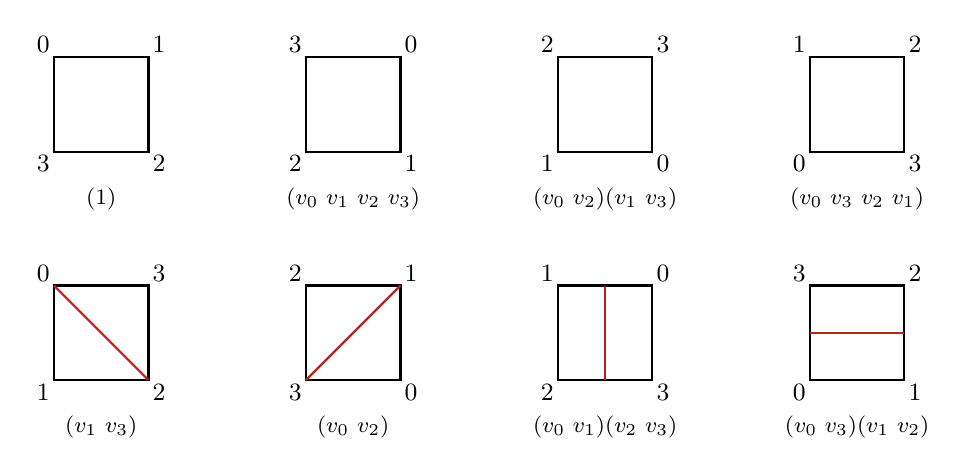
\begin{tikzpicture}[scale=1]
		% #1,#2: position; #3-#6: labels at top-left, top-right, bottom-right,
		% bottom-left; #7: extra drawing (reflection axis); #8: the permutation
		\newcommand{\dsq}[8]{%
			\begin{scope}[shift={(#1,#2)}]
				\draw[thick] (0,0) rectangle (1.2,1.2);
				#7
				\node[above left=-2pt]  at (0,1.2)   {\small #3};
				\node[above right=-2pt] at (1.2,1.2) {\small #4};
				\node[below right=-2pt] at (1.2,0)   {\small #5};
				\node[below left=-2pt]  at (0,0)     {\small #6};
				\node at (0.6,-0.6) {\footnotesize #8};
			\end{scope}}
		\dsq{0}{2.9}{0}{1}{2}{3}{}{\((1)\)}
		\dsq{3.2}{2.9}{3}{0}{1}{2}{}{\((v_0\ v_1\ v_2\ v_3)\)}
		\dsq{6.4}{2.9}{2}{3}{0}{1}{}{\((v_0\ v_2)(v_1\ v_3)\)}
		\dsq{9.6}{2.9}{1}{2}{3}{0}{}{\((v_0\ v_3\ v_2\ v_1)\)}
		\dsq{0}{0}{0}{3}{2}{1}{\draw[BrickRed, thick] (0,1.2) -- (1.2,0);}{\((v_1\ v_3)\)}
		\dsq{3.2}{0}{2}{1}{0}{3}{\draw[BrickRed, thick] (0,0) -- (1.2,1.2);}{\((v_0\ v_2)\)}
		\dsq{6.4}{0}{1}{0}{3}{2}{\draw[BrickRed, thick] (0.6,0) -- (0.6,1.2);}{\((v_0\ v_1)(v_2\ v_3)\)}
		\dsq{9.6}{0}{3}{2}{1}{0}{\draw[BrickRed, thick] (0,0.6) -- (1.2,0.6);}{\((v_0\ v_3)(v_1\ v_2)\)}
	\end{tikzpicture}
	\caption{The dihedral group \(D_8\) acting on the vertices of a square. Label \(i\)
		marks where the vertex \(v_i\) is sent; the top row shows the rotations, the bottom
		row the reflections (with their axes).}
	\label{fig:D8-action}
\end{figure}

\begin{eg}[\(D_8\) acting on a square]\label{eg:D8-square}
	Let \(X = \{v_0, v_1, v_2, v_3\}\) be the vertices of a square (labelled as in
	\autoref{fig:regular-polygons}), and let \(G = D_8\) act on \(X\) as in
	\autoref{fig:D8-action}:
	\begin{align*}
		G = \{ & \text{rotations: } (1),\ (v_0\ v_1\ v_2\ v_3),\ (v_0\ v_2)(v_1\ v_3),\
		(v_0\ v_3\ v_2\ v_1);                                                        \\
		       & \text{reflections: } (v_1\ v_3),\ (v_0\ v_2),\ (v_0\ v_1)(v_2\ v_3),\
		(v_0\ v_3)(v_1\ v_2)\}.
	\end{align*}
	For each vertex \(v_i\) there is some \(g \in G\) with \(gv_0 = v_i\) (a rotation will
	do); therefore \(\mathcal O(v_0) = X\), and \(D_8\) acts transitively.

	What is the stabilizer \(G_{v_0}\)? Aside from the identity, there is only one
	\(g \in D_8\) fixing \(v_0\), namely \(g = (v_1\ v_3)\); therefore \(G_{v_0}\) is a
	subgroup of order \(2\). (This generalizes to \(D_{2n}\) acting on the vertices of a
	regular \(n\)-gon: the action is transitive, and the stabilizer of \(v_0\) is
	\(\{1, b\}\), where \(b\) is the reflection with axis \(L[O,v_0]\).)
\end{eg}

\begin{eg}[Conjugacy classes and centralizers]\label{eg:conjugacy-class}
	Let a group \(G\) act on itself by conjugation. If \(x \in G\), then
	\[
		\mathcal O(x) = \{y \in G : y = axa^{-1} \text{ for some } a \in G\};
	\]
	\(\mathcal O(x)\) is called the \vocab{conjugacy class} of \(x\), and it is often
	denoted by \(x^G\). For example, \autoref{prop:conjugacy-criterion} shows that if
	\(\alpha \in S_n\), then the conjugacy class of \(\alpha\) consists of all the
	permutations in \(S_n\) having the same cycle structure as \(\alpha\).

	If \(x \in G\), then the stabilizer \(G_x\) of \(x\) is
	\[
		C_G(x) = \{g \in G : gxg^{-1} = x\}.
	\]
	This subgroup of \(G\), consisting of all \(g \in G\) that commute with \(x\), is
	called the \vocab{centralizer} of \(x\) in \(G\).
\end{eg}

\begin{eg}[A cyclic subgroup of \(S_n\)]\label{eg:cyclic-perm-action}
	Let \(X = \{1, 2, \dots, n\}\), let \(\sigma \in S_n\), and let the cyclic group
	\(G = \langle\sigma\rangle\) act on \(X\). If \(i \in X\), then
	\[
		\mathcal O(i) = \{\sigma^k(i) : k \in \mathbb Z\}.
	\]
	Let \(\sigma = \beta_1\cdots\beta_{t}\) be the complete factorization of \(\sigma\),
	and suppose the cycle containing \(i = i_1\) is \(\beta_j = (i_1\ i_2\ \dots\ i_r)\).
	As in the proof of \autoref{prop:disjoint-cycles}, \(\sigma^k(i_1) = i_{k+1}\) for
	\(0 \leq k \leq r-1\), while \(\sigma^r(i_1) = i_1\); so the powers \(\sigma^k(i_1)\)
	run cyclically through \(i_1, \dots, i_r\). Therefore
	\[
		\mathcal O(i) = \{i_1, i_2, \dots, i_r\}, \qquad \abs{\mathcal O(i)} = r.
	\]
	The stabilizer \(G_\ell\) of a symbol \(\ell\) is all of \(G\) if \(\sigma\) fixes
	\(\ell\), and it is a proper subgroup of \(G\) if \(\sigma\) moves \(\ell\) (for then
	\(\sigma \notin G_\ell\)).
\end{eg}

A group \(G\) acting on a set \(X\) gives an equivalence relation on \(X\): define
\[
	x \equiv y \quad\text{if there exists } g \in G \text{ with } y = gx.
\]
\emph{Reflexive:} \(x = 1x\). \emph{Symmetric:} if \(y = gx\), then
\(g^{-1}y = g^{-1}(gx) = (g^{-1}g)x = x\), so \(y \equiv x\). \emph{Transitive:} if
\(y = gx\) and \(z = hy\), then \(z = h(gx) = (hg)x\), so \(x \equiv z\). The equivalence
class of \(x \in X\) is exactly its orbit:
\[
	[x] = \{y \in X : y \equiv x\} = \{gx : g \in G\} = \mathcal O(x).
\]

\begin{proposition}\label{prop:orbits-partition}
	If \(G\) acts on a set \(X\), then \(X\) is the disjoint union of the orbits. If \(X\)
	is finite, then
	\[
		\abs{X} = \sum_i \abs{\mathcal O(x_i)},
	\]
	where one \(x_i\) is chosen from each orbit.
\end{proposition}

\begin{proof}
	The orbits are the equivalence classes of \(\equiv\), and the equivalence classes of an
	equivalence relation form a partition of \(X\). The count is correct because the orbits
	are disjoint, so no element of \(X\) is counted twice.
\end{proof}

Here is the connection between orbits and stabilizers.

\begin{theorem}[Orbit--stabilizer]\label{thm:orbit-stabilizer}
	If \(G\) acts on a set \(X\) and \(x \in X\), then
	\[
		\abs{\mathcal O(x)} = [G : G_x],
	\]
	the index of the stabilizer \(G_x\) in \(G\).
\end{theorem}

\begin{proof}
	Let \(G/G_x\) denote the family of all cosets of \(G_x\) in \(G\). We exhibit a
	bijection \(\varphi\colon \mathcal O(x) \to G/G_x\); this gives the result, since
	\(\abs{G/G_x} = [G : G_x]\) by definition of the index.

	If \(y \in \mathcal O(x)\), then \(y = gx\) for some \(g \in G\); define
	\(\varphi(y) = gG_x\).
	\begin{itemize}
		\item \emph{Well defined:} if also \(y = hx\), then \(h^{-1}gx = h^{-1}y = x\), so
		      \(h^{-1}g \in G_x\), and \(hG_x = gG_x\) by \autoref{lem:coset-basics}(i).
		\item \emph{Injective:} suppose \(\varphi(y) = \varphi(z)\), where \(y = gx\),
		      \(z = hx\), and \(gG_x = hG_x\). Then \(h^{-1}g \in G_x\), so
		      \(h^{-1}gx = x\); applying \(h\) gives \(y = gx = hx = z\).
		\item \emph{Surjective:} given \(gG_x \in G/G_x\), let \(y = gx \in \mathcal O(x)\);
		      then \(\varphi(y) = gG_x\). \qedhere
	\end{itemize}
\end{proof}

\begin{eg}
	In \autoref{eg:D8-square}, \(D_8\) acting on the four corners of a square, we saw
	\(\abs{\mathcal O(v_0)} = 4\), \(\abs{G_{v_0}} = 2\), and indeed
	\([G : G_{v_0}] = 8/2 = 4\).

	In \autoref{eg:cyclic-perm-action}, \(G = \langle\sigma\rangle \leq S_n\) acting on
	\(X = \{1, \dots, n\}\), if an \(r\)-cycle \(\beta_j\) in the complete factorization of
	\(\sigma\) moves \(\ell\), then \(r = \abs{\mathcal O(\ell)}\).
	\autoref{thm:orbit-stabilizer} says that \(r\) divides \(\abs{G}\), which is the order
	\(k\) of \(\sigma\). (\autoref{prop:order-permutation} tells us more: \(k\) is the lcm
	of the lengths of the cycles in the factorization.)
\end{eg}

\begin{corollary}\label{cor:orbit-divides}
	If a finite group \(G\) acts on a set \(X\), then the number of elements in any orbit
	is a divisor of \(\abs{G}\).
\end{corollary}

\begin{proof}
	\(\abs{\mathcal O(x)} = [G : G_x] = \abs{G}/\abs{G_x}\), by
	\autoref{thm:orbit-stabilizer} and \autoref{cor:index-formula}.
\end{proof}

\begin{corollary}\label{cor:class-size}
	If \(x\) lies in a finite group \(G\), then the number of conjugates of \(x\) is the
	index of its centralizer:
	\[
		\abs{x^G} = [G : C_G(x)],
	\]
	and hence it is a divisor of \(\abs{G}\).
\end{corollary}

\begin{proof}
	As in \autoref{eg:conjugacy-class}, for the conjugation action the orbit of \(x\) is
	its conjugacy class \(x^G\), and the stabilizer \(G_x\) is the centralizer
	\(C_G(x)\).
\end{proof}

In \autoref{tab:cycle-counts} we counted the permutations in \(S_4\) of each cycle
structure: \(1, 6, 8, 6, 3\). Each of these numbers divides \(\abs{S_4} = 24\). The
corresponding numbers for \(S_5\) are \(1, 10, 20, 30, 24, 20, 15\), and these all divide
\(\abs{S_5} = 120\). We now recognize these subsets as conjugacy classes, and the next
corollary explains why these numbers divide the group order.

\begin{corollary}\label{cor:cycle-structure-count}
	If \(\alpha \in S_n\), then the number of permutations in \(S_n\) having the same cycle
	structure as \(\alpha\) is a divisor of \(n!\).
\end{corollary}

\begin{proof}
	By \autoref{prop:conjugacy-criterion}, two permutations in \(S_n\) are conjugate if
	and only if they have the same cycle structure. So the permutations with the cycle
	structure of \(\alpha\) form the conjugacy class \(\alpha^{S_n}\), whose size divides
	\(\abs{S_n} = n!\) by \autoref{cor:class-size}.
\end{proof}

\subsection{Cauchy's Theorem and \(p\)-Groups}

When we classified groups of order \(6\), it would have been helpful to know that any such
group has an element of order \(3\) (we could only use \autoref{lem:even-order} to find
an element of order \(2\)). We now prove that every finite group \(G\) contains an element
of prime order \(p\) for every prime \(p \mid \abs{G}\).

If the conjugacy class \(x^G\) of an element \(x\) consists of \(x\) alone, then
\(gxg^{-1} = x\), that is, \(gx = xg\), for every \(g \in G\); so \(x \in Z(G)\).
Conversely, if \(x \in Z(G)\), then \(x^G = \{x\}\). Thus
\[
	Z(G) = \{x \in G : \abs{x^G} = 1\}.
\]

\begin{theorem}[Cauchy]\label{thm:cauchy}
	If \(G\) is a finite group whose order is divisible by a prime \(p\), then \(G\)
	contains an element of order \(p\).
\end{theorem}

\begin{proof}
	We prove the theorem by induction on \(\abs{G}\); the base step \(\abs{G} = 1\) is
	vacuously true, for there are no prime divisors of \(1\).

	If \(x \in G\), then the number of conjugates of \(x\) is
	\(\abs{x^G} = [G : C_G(x)]\) by \autoref{cor:class-size}. If \(x \notin Z(G)\), then
	\(x^G\) has more than one element, and so \(\abs{C_G(x)} < \abs{G}\). If
	\(p \mid \abs{C_G(x)}\) for some noncentral \(x\), then the inductive hypothesis gives
	an element of order \(p\) in \(C_G(x) \leq G\), and we are done. Therefore we may
	assume that \(p \nmid \abs{C_G(x)}\) for all noncentral \(x \in G\). Better, since
	\(\abs{G} = [G : C_G(x)]\,\abs{C_G(x)}\) is divisible by \(p\), Euclid's lemma gives
	\[
		p \mid [G : C_G(x)] \quad\text{for every noncentral } x.
	\]

	Now apply \autoref{prop:orbits-partition} to the conjugation action. The orbits of
	size \(1\) are exactly the singletons \(\{z\}\) with \(z \in Z(G)\), and there are
	\(\abs{Z(G)}\) of them; so
	\[
		\abs{G} = \abs{Z(G)} + \sum_i [G : C_G(x_i)],
	\]
	where one \(x_i\) is selected from each conjugacy class having more than one element.
	Since \(\abs{G}\) and all \([G : C_G(x_i)]\) are divisible by \(p\), it follows that
	\(\abs{Z(G)}\) is divisible by \(p\). But \(Z(G)\) is abelian, so
	\autoref{prop:hom-facts}(vi) says that \(Z(G)\), and hence \(G\), contains an element
	of order \(p\).
\end{proof}

\begin{remark}
	The proof uses the abelian case of Cauchy's theorem, which was proved in Rotman §2.6
	with quotient groups. \autoref{eg:mckay} below gives a completely independent proof.
\end{remark}

\begin{definition}[Class equation]\label{def:class-equation}
	The \vocab{class equation} of a finite group \(G\) is
	\[
		\abs{G} = \abs{Z(G)} + \sum_i [G : C_G(x_i)],
	\]
	where one \(x_i\) is selected from each conjugacy class having more than one element.
\end{definition}

\begin{eg}
	In \(S_3\) the center is trivial, and the other conjugacy classes are the transpositions
	and the \(3\)-cycles, so the class equation is \(6 = 1 + 3 + 2\). In \(S_4\),
	\autoref{tab:cycle-counts} gives \(24 = 1 + 6 + 8 + 6 + 3\).
\end{eg}

\begin{definition}[\(p\)-group]
	If \(p\) is a prime, then a \vocab{\(p\)-group} is a group of order \(p^n\) for some
	\(n \geq 0\).
\end{definition}

There are groups whose center is trivial; for example, \(Z(S_3) = \{1\}\). For
\(p\)-groups with more than one element, however, this never happens.

\begin{theorem}\label{thm:p-group-center}
	If \(p\) is a prime and \(G\) is a \(p\)-group with more than one element, then
	\(Z(G) \neq \{1\}\).
\end{theorem}

\begin{proof}
	Consider the class equation
	\[
		\abs{G} = \abs{Z(G)} + \sum_i [G : C_G(x_i)].
	\]
	Each \(C_G(x_i)\) is a proper subgroup of \(G\), for \(x_i \notin Z(G)\). Since
	\([G : C_G(x_i)]\) is a divisor of \(\abs{G}\), a power of \(p\), it is itself a power of
	\(p\), and it is not \(p^0 = 1\). Thus \(p\) divides \(\abs{G}\) and each term of the
	sum, and so \(p \mid \abs{Z(G)}\) as well. Therefore \(\abs{Z(G)} \geq p\), and
	\(Z(G) \neq \{1\}\).
\end{proof}

\begin{corollary}\label{cor:p2-abelian}
	If \(p\) is a prime, then every group \(G\) of order \(p^2\) is abelian.
\end{corollary}

\begin{proof}
	If \(G\) is not abelian, then \(Z(G)\) is a proper subgroup, so
	\(\abs{Z(G)} = 1\) or \(p\) by Lagrange's theorem. But \(Z(G) \neq \{1\}\) by
	\autoref{thm:p-group-center}, so \(\abs{Z(G)} = p\). The center is a normal subgroup,
	so the quotient \(G/Z(G)\) is defined; it has order \(p\), hence is cyclic. Then
	\autoref{lem:center-cyclic} says \(G\) is abelian, a contradiction.
\end{proof}

\begin{eg}[Nonabelian groups of order \(p^3\)]\label{eg:UT3p}
	For every prime \(p\), there exist nonabelian groups of order \(p^3\). Let
	\(UT(3,p)\) be the set of all upper triangular \(3 \times 3\) matrices over
	\(\mathbb Z_p\) with \(1\)'s on the diagonal:
	\[
		UT(3,p) = \left\{
		\begin{pmatrix} 1 & a & b \\ 0 & 1 & c \\ 0 & 0 & 1 \end{pmatrix}
		: a, b, c \in \mathbb Z_p \right\}.
	\]
	It is a subgroup of \(GL(3,\mathbb Z_p)\): it contains \(I\), and
	\begin{gather*}
		\begin{pmatrix} 1 & a & b \\ 0 & 1 & c \\ 0 & 0 & 1 \end{pmatrix}
		\begin{pmatrix} 1 & a' & b' \\ 0 & 1 & c' \\ 0 & 0 & 1 \end{pmatrix}
		= \begin{pmatrix} 1 & a+a' & b+ac'+b' \\ 0 & 1 & c+c' \\ 0 & 0 & 1 \end{pmatrix},
		\\
		\begin{pmatrix} 1 & a & b \\ 0 & 1 & c \\ 0 & 0 & 1 \end{pmatrix}^{-1}
		= \begin{pmatrix} 1 & -a & ac-b \\ 0 & 1 & -c \\ 0 & 0 & 1 \end{pmatrix}.
	\end{gather*}
	It has order \(p^3\), because there are \(p\) choices for each of \(a, b, c\). It is
	not abelian: by the product formula, the matrices with \((a,b,c) = (1,0,0)\) and
	\((0,0,1)\) multiply to \((1,1,1)\) in one order and to \((1,0,1)\) in the other.
	(Rotman, Exercise 2.111: \(UT(3,2) \cong D_8\).)
\end{eg}

\begin{eg}[McKay's proof of Cauchy's and Fermat's theorems]\label{eg:mckay}
	Who would have guessed that Cauchy's theorem and Fermat's theorem are special cases of
	a common theorem? The following elementary yet ingenious proof is due to J.~H.~McKay.

	Let \(G\) be a finite group and \(p\) a prime, and let
	\[
		X = \{(a_1, a_2, \dots, a_p) \in G^p : a_1a_2\cdots a_p = 1\},
	\]
	where \(G^p\) is the cartesian product of \(p\) copies of \(G\). Then
	\(\abs{X} = \abs{G}^{p-1}\): having chosen the first \(p-1\) entries arbitrarily, the
	\(p\)th entry must equal \((a_1a_2\cdots a_{p-1})^{-1}\).

	Make \(X\) into a \(\mathbb Z_p\)-set by cyclically shifting: for
	\(0 \leq i \leq p-1\),
	\[
		[i](a_1, a_2, \dots, a_p) = (a_{i+1}, a_{i+2}, \dots, a_p, a_1, a_2, \dots, a_i).
	\]
	(Shifting by \(j\) and then by \(i\) is shifting by \(i+j\), so this is an action.)
	The shifted tuple lies in \(X\), because the product of its entries is a conjugate of
	\(a_1a_2\cdots a_p = 1\):
	\[
		a_{i+1}\cdots a_pa_1\cdots a_i
		= (a_1\cdots a_i)^{-1}(a_1a_2\cdots a_p)(a_1\cdots a_i) = 1.
	\]
	By \autoref{cor:orbit-divides}, every orbit has size dividing
	\(\abs{\mathbb Z_p} = p\), so its size is \(1\) or \(p\). An orbit has size \(1\)
	exactly when the tuple is unchanged by the shift \([1]\), that is, when all its entries
	are equal: \((a, a, \dots, a)\), which lies in \(X\) if and only if \(a^p = 1\). So if
	\(s = \abs{\{a \in G : a^p = 1\}}\), then \autoref{prop:orbits-partition} gives
	\[
		\abs{G}^{p-1} = \abs{X} = s + kp \quad\text{for some } k \geq 0.
	\]
	\begin{itemize}
		\item \emph{Cauchy.} If \(p \mid \abs{G}\), then \(p \mid s\). Since \(s \geq 1\)
		      (take \(a = 1\)), we get \(s \geq p \geq 2\), so some \(a \neq 1\) satisfies
		      \(a^p = 1\); such an \(a\) has order \(p\).
		\item \emph{Fermat.} Let \(G = \mathbb Z_n\) with \(n \geq 1\) (written
		      additively, so ``\(a^p = 1\)'' reads \(pa = 0\)). If \(p \nmid n\), then an
		      element with \(pa = 0\) has order dividing both \(p\) and \(n\)
		      (\autoref{lem:order-divides} and \autoref{cor:order-divides-group}), so
		      \(a = 0\) and \(s = 1\). Hence \(n^{p-1} = 1 + kp\), i.e.\
		      \(n^{p-1} \equiv 1 \pmod p\), and multiplying by \(n\) gives
		      \(n^p \equiv n \pmod p\). This congruence also holds when \(p \mid n\), both
		      sides being \(\equiv 0\). Since both sides depend only on \(n \bmod p\), it
		      holds for every integer \(n\): this is \vocab{Fermat's theorem}.
	\end{itemize}
\end{eg}

\begin{remark}
	The argument proves more: if \(\abs{G} = n\), then the number of solutions of
	\(x^p = 1\) in \(G\) is \(s \equiv n^{p-1} \pmod p\).
\end{remark}

We have seen that \(A_4\) is a group of order \(12\) having no subgroup of order \(6\). So
the converse of Lagrange's theorem is false. It is true, however, when \(G\) is a
\(p\)-group; indeed, more is true.

\begin{proposition}\label{prop:p-group-normal-subgroups}
	If \(G\) is a group of order \(p^e\), then \(G\) has a normal subgroup of order \(p^k\)
	for every \(k \leq e\).
\end{proposition}

\begin{proof}
	We induct on \(e \geq 0\). The base step \(e = 0\) is obvious (take \(\{1\}\)), so
	assume \(e \geq 1\). By \autoref{thm:p-group-center}, \(Z(G) \neq \{1\}\).

	If \(Z(G) = G\), then \(G\) is abelian; \autoref{prop:hom-facts}(vi) gives a subgroup
	of order \(p^k\), and it is normal because \(G\) is abelian.

	Assume that \(Z(G)\) is a proper subgroup, say \(\abs{Z(G)} = p^c\) with
	\(1 \leq c < e\). If \(k \leq c\), then the abelian group \(Z(G)\) contains a subgroup
	of order \(p^k\) by \autoref{prop:hom-facts}(vi), and this subgroup is normal in \(G\)
	since it lies in the center (\autoref{prop:hom-facts}(ii)). If \(k > c\), consider
	\(G/Z(G)\), a \(p\)-group of order \(p^{e-c} < p^e\). By induction it contains a
	normal subgroup \(S^*\) of order \(p^{k-c}\). The correspondence theorem gives a
	normal subgroup \(S\) of \(G\) with
	\[
		Z(G) \leq S \trianglelefteq G \qquad\text{and}\qquad S/Z(G) = S^*.
	\]
	Then \(\abs{S} = [S : Z(G)]\,\abs{Z(G)} = \abs{S^*}\,\abs{Z(G)}
	= p^{k-c}\cdot p^c = p^k\).
\end{proof}

\subsection{Simple Groups}

Abelian groups (and the quaternions) have the property that every subgroup is normal. At
the opposite pole are the groups having no normal subgroups other than the two obvious
ones, \(\{1\}\) and \(G\).

\begin{definition}[Simple group]
	A group \(G\) is \vocab{simple} if \(G \neq \{1\}\) and \(G\) has no normal subgroups
	other than \(\{1\}\) and \(G\) itself.
\end{definition}

\begin{proposition}\label{prop:abelian-simple}
	An abelian group \(G\) is simple if and only if it is finite of prime order.
\end{proposition}

\begin{proof}
	If \(G\) is finite of prime order \(p\), then \(G\) has no subgroups \(H\) other than
	\(\{1\}\) and \(G\), since \(\abs{H}\) divides \(p\) by Lagrange's theorem. Therefore
	\(G\) is simple.

	Conversely, assume that \(G\) is simple. Since \(G\) is abelian, every subgroup is
	normal, so \(G\) has no subgroups other than \(\{1\}\) and \(G\). Choose \(x \in G\)
	with \(x \neq 1\); since \(\langle x\rangle \neq \{1\}\), we have
	\(\langle x\rangle = G\). If \(x\) had infinite order, then all powers of \(x\) would be
	distinct, and \(\langle x^2\rangle\) would be a subgroup with
	\(\{1\} \neq \langle x^2\rangle \neq \langle x\rangle\) (as \(x \notin \langle x^2\rangle\)), a
	contradiction. So \(x\) has finite order \(m\), and \(\abs{G} = m\). If \(m\) were
	composite, say \(m = k\ell\) with \(1 < k < m\), then \(\langle x^k\rangle\) would be a
	subgroup of order \(\ell\), neither \(\{1\}\) nor \(G\), a contradiction. Therefore
	\(G = \langle x\rangle\) has prime order.
\end{proof}

We are now going to show that \(A_5\) is a nonabelian simple group; indeed, it is the
smallest one, for there is no nonabelian simple group of order less than \(60\).

Suppose that \(x \in G\) has \(k\) conjugates: \(\abs{x^G} = k\). If \(H\) is a subgroup
with \(x \in H \leq G\), how many conjugates does \(x\) have in \(H\)? Since
\[
	x^H = \{hxh^{-1} : h \in H\} \subseteq \{gxg^{-1} : g \in G\} = x^G,
\]
we have \(\abs{x^H} \leq \abs{x^G}\), and the inequality can be strict. For example, take
\(G = S_3\), \(x = (1\ 2)\), and \(H = \langle x\rangle\): then \(\abs{x^G} = 3\) (all
transpositions are conjugate), whereas \(\abs{x^H} = 1\) (because \(H\) is abelian). Let us
consider this question for \(G = S_5\), \(x = (1\ 2\ 3)\), and \(H = A_5\).

\begin{lemma}\label{lem:A5-3-cycles-conjugate}
	All \(3\)-cycles are conjugate in \(A_5\).
\end{lemma}

\begin{proof}
	Let \(\alpha = (1\ 2\ 3)\). There are \(20\) \(3\)-cycles in \(S_5\)
	(\autoref{tab:cycle-counts}), and they are all conjugate in \(S_5\), so
	\(\abs{\alpha^{S_5}} = 20\). By \autoref{cor:class-size},
	\(20 = \abs{S_5}/\abs{C_{S_5}(\alpha)} = 120/\abs{C_{S_5}(\alpha)}\), so
	\(\abs{C_{S_5}(\alpha)} = 6\): there are exactly six permutations in \(S_5\) commuting
	with \(\alpha\). Here they are:
	\[
		(1), \quad (1\ 2\ 3), \quad (1\ 3\ 2), \quad (4\ 5), \quad
		(4\ 5)(1\ 2\ 3), \quad (4\ 5)(1\ 3\ 2).
	\]
	The last three are odd, so \(C_{A_5}(\alpha) = C_{S_5}(\alpha) \cap A_5\) has order
	\(3\). We conclude that
	\[
		\abs{\alpha^{A_5}} = \abs{A_5}/\abs{C_{A_5}(\alpha)} = 60/3 = 20;
	\]
	that is, all twenty \(3\)-cycles are conjugate to \(\alpha\) in \(A_5\), hence to each
	other.
\end{proof}

\begin{lemma}\label{lem:products-of-3-cycles}
	If \(n \geq 3\), then every element of \(A_n\) is a \(3\)-cycle or a product of
	\(3\)-cycles.
\end{lemma}

\begin{proof}
	The identity is \((1\ 2\ 3)^3\). If \(\alpha \in A_n\), then \(\alpha\) is a product of
	an even number of transpositions, \(\alpha = \tau_1\tau_2\cdots\tau_{2m-1}\tau_{2m}\)
	(\autoref{thm:parity}). Grouping the transpositions in pairs \(\tau_{2i-1}\tau_{2i}\),
	it suffices to consider a product \(\tau\tau'\) of two transpositions. If
	\(\tau = \tau'\), then \(\tau\tau' = (1)\), which can be dropped. If \(\tau\) and
	\(\tau'\) share exactly one symbol, then \(\tau = (i\ j)\), \(\tau' = (i\ k)\), and
	\(\tau\tau' = (i\ k\ j)\). If they are disjoint, then
	\[
		\tau\tau' = (i\ j)(k\ \ell) = (i\ j)(j\ k)(j\ k)(k\ \ell) = (i\ j\ k)(j\ k\ \ell).
		\qedhere
	\]
\end{proof}

\begin{theorem}\label{thm:A5-simple}
	\(A_5\) is a simple group.
\end{theorem}

\begin{proof}
	We show that if \(H \trianglelefteq A_5\) and \(H \neq \{(1)\}\), then \(H = A_5\). If
	\(H\) contains a \(3\)-cycle, then normality forces \(H\) to contain all its conjugates
	in \(A_5\), so \(H\) contains every \(3\)-cycle by
	\autoref{lem:A5-3-cycles-conjugate}, and \(H = A_5\) by
	\autoref{lem:products-of-3-cycles}. Therefore it suffices to prove that \(H\) contains
	a \(3\)-cycle.

	As \(H \neq \{(1)\}\), it contains some \(\sigma \neq (1)\). The even cycle structures
	in \(S_5\) are those of \((1)\), \((1\ 2\ 3)\), \((1\ 2)(3\ 4)\), and
	\((1\ 2\ 3\ 4\ 5)\), so \(\sigma\) is a \(3\)-cycle (and we are done), or
	\(\sigma = (a\ b)(c\ d)\), or \(\sigma = (a\ b\ c\ d\ e)\); in either of the last two
	cases write \(\{a, b, c, d, e\} = \{1, 2, 3, 4, 5\}\).
	\begin{itemize}
		\item If \(\sigma = (a\ b)(c\ d) \in H\), conjugate by \(\beta = (c\ d\ e) \in A_5\):
		      by \autoref{prop:conj-same-structure},
		      \(\sigma' = \beta\sigma\beta^{-1} = (a\ b)(d\ e) \in H\), because
		      \(H \trianglelefteq A_5\). Hence
		      \(\sigma\sigma' = (c\ d)(d\ e) = (c\ d\ e) \in H\).
		\item If \(\sigma = (a\ b\ c\ d\ e) \in H\), conjugate by
		      \(\gamma = (a\ b\ c) \in A_5\):
		      \(\sigma'' = \gamma\sigma\gamma^{-1} = (b\ c\ a\ d\ e) \in H\). Hence
		      \[
			      \sigma''\sigma^{-1} = (b\ c\ a\ d\ e)(e\ d\ c\ b\ a) = (a\ b\ d) \in H.
		      \]
	\end{itemize}
	In all cases \(H\) contains a \(3\)-cycle. Therefore the only normal subgroups of \(A_5\)
	are \(\{(1)\}\) and \(A_5\) itself, and \(A_5\) is simple.
\end{proof}

\begin{remark}
	Where did the last computation come from? If \(\sigma \in H\) and \(\gamma\) is a
	\(3\)-cycle, then \(\gamma\sigma\gamma^{-1} \in H\), so
	\((\gamma\sigma\gamma^{-1})\sigma^{-1} = \gamma(\sigma\gamma^{-1}\sigma^{-1}) \in H\).
	But \(\sigma\gamma^{-1}\sigma^{-1}\) is a \(3\)-cycle, so \(H\) contains a product of
	two \(3\)-cycles. We chose \(\gamma\) carefully to force this product to be a
	\(3\)-cycle. The same trick drives the proof of \autoref{thm:An-simple}.
\end{remark}

\begin{remark}
	As we shall see in Chapter 5, \autoref{thm:A5-simple} turns out to be the basic reason
	why the quadratic formula has no generalization giving the roots of polynomials of
	degree \(5\) or higher.
\end{remark}

Observe that \(A_4\) is \emph{not} simple: the four-group \(\mathbf V\) consists of
\((1)\) and the three permutations in \(S_4\) of cycle structure \((a\ b)(c\ d)\), all of
which are even; since conjugation preserves cycle structure
(\autoref{prop:conj-same-structure}), \(g\mathbf Vg^{-1} = \mathbf V\) for all
\(g \in S_4\). Thus \(\{(1)\} \neq \mathbf V \trianglelefteq A_4\), and
\(\mathbf V \neq A_4\). Without much more effort, however, we can prove that \(A_n\) is
simple for every \(n \geq 5\). We first generalize the two lemmas used for \(A_5\).

\begin{lemma}[Rotman, Exercise 2.116]\label{lem:An-3-cycles}
	Let \(n \geq 5\).
	\begin{enumerate}[(i)]
		\item All \(3\)-cycles are conjugate in \(A_n\).
		\item If \(H \trianglelefteq A_n\) contains a \(3\)-cycle, then \(H = A_n\).
	\end{enumerate}
\end{lemma}

\begin{proof}
	(i) Let \(\gamma, \gamma'\) be \(3\)-cycles. By \autoref{prop:conjugacy-criterion}
	there is \(\alpha \in S_n\) with \(\alpha\gamma\alpha^{-1} = \gamma'\). If \(\alpha\) is
	even we are done. If \(\alpha\) is odd, choose two symbols \(k, \ell\) fixed by
	\(\gamma\) (possible since \(n \geq 5\)) and let \(\tau = (k\ \ell)\). Then \(\tau\)
	and \(\gamma\) are disjoint, so they commute (\autoref{lem:disjoint-commute}), and
	\(\alpha\tau\) is even with
	\[
		(\alpha\tau)\gamma(\alpha\tau)^{-1} = \alpha(\tau\gamma\tau^{-1})\alpha^{-1}
		= \alpha\gamma\alpha^{-1} = \gamma'.
	\]

	(ii) By normality and (i), \(H\) contains every \(3\)-cycle, so \(H = A_n\) by
	\autoref{lem:products-of-3-cycles}.
\end{proof}

\begin{lemma}[Rotman, Exercise 2.118]\label{lem:F-iso-Ar}
	Let \(Y = \{i_1, \dots, i_r\} \subseteq \{1, 2, \dots, n\}\), and let
	\[
		F = \{\sigma \in A_n : \sigma \text{ fixes every } i \notin Y\}.
	\]
	Then \(F\) is a subgroup of \(A_n\) and \(F \cong A_r\).
\end{lemma}

\begin{proof}
	Let \(E = \{\sigma \in S_n : \sigma \text{ fixes every } i \notin Y\}\). If
	\(\sigma \in E\), then \(\sigma\) maps the complement of \(Y\) onto itself, hence (being
	a bijection) maps \(Y\) onto \(Y\); so the restriction \(\sigma|_Y\) lies in \(S_Y\).
	The map \(E \to S_Y\), \(\sigma \mapsto \sigma|_Y\), is a homomorphism (restricting a
	composite gives the composite of restrictions, as \(\sigma(Y) = Y\)); it is injective,
	since \(\sigma\) is known off \(Y\); and it is surjective, since every \(\pi \in S_Y\)
	extends by the identity to an element of \(E\). So \(E \cong S_Y\).

	This isomorphism preserves parity: if \(\pi \in S_Y\) has a complete factorization with
	\(t\) cycles, then its extension has the same cycles plus \(n - r\) extra \(1\)-cycles,
	so its signum is \((-1)^{n-(t+n-r)} = (-1)^{r-t} = \sgn(\pi)\). Hence
	\(F = E \cap A_n\) corresponds to the even permutations of \(Y\), and
	\(F \cong A_Y \cong A_r\), the last isomorphism by \autoref{lem:SX-iso} (which preserves
	parity). In particular \(F\), being the image of a subgroup under an isomorphism, is a
	subgroup.
\end{proof}

\begin{lemma}\label{lem:A6-simple}
	\(A_6\) is a simple group.
\end{lemma}

\begin{proof}
	Let \(H \neq \{(1)\}\) be a normal subgroup of \(A_6\); we must show \(H = A_6\).

	Assume first that some \(\alpha \in H\) with \(\alpha \neq (1)\) fixes some \(i\),
	\(1 \leq i \leq 6\). Define
	\[
		F = \{\sigma \in A_6 : \sigma(i) = i\}.
	\]
	Then \(\alpha \in H \cap F\), so \(H \cap F \neq \{(1)\}\). Moreover
	\(H \cap F \trianglelefteq F\): if \(\sigma \in F\) and \(h \in H \cap F\), then
	\(\sigma h\sigma^{-1} \in H\) (as \(H \trianglelefteq A_6\)) and
	\(\sigma h\sigma^{-1} \in F\). But \(F \cong A_5\) by \autoref{lem:F-iso-Ar}, so \(F\)
	is simple by \autoref{thm:A5-simple}, and hence \(H \cap F = F\); that is,
	\(F \leq H\). Now \(F\) contains \(3\)-cycles (any \(3\)-cycle not involving \(i\)), so
	\(H\) contains a \(3\)-cycle, and \(H = A_6\) by \autoref{lem:An-3-cycles}.

	We may now assume that no \(\alpha \in H\) with \(\alpha \neq (1)\) fixes any \(i\).
	An even permutation of six symbols fixing none of them has cycle structure
	\((1\ 2)(3\ 4\ 5\ 6)\) or \((1\ 2\ 3)(4\ 5\ 6)\) (the structures \((1\ 2\ \dots\ 6)\)
	and \((1\ 2)(3\ 4)(5\ 6)\) are odd). In the first case, say
	\(\alpha = (a\ b)(c\ d\ e\ f)\), the element
	\(\alpha^2 = (c\ e)(d\ f) \in H\) is nontrivial and fixes \(a\), a contradiction. In
	the second case, say \(\alpha = (1\ 2\ 3)(4\ 5\ 6)\) after renaming, let
	\(\beta = (2\ 3\ 4)\). Then \(\beta\alpha^{-1}\beta^{-1} \in H\) by normality, and
	\(\beta\alpha^{-1}\beta^{-1} = (1\ 4\ 3)(2\ 6\ 5)\) by
	\autoref{prop:conj-same-structure}, so
	\[
		\alpha(\beta\alpha^{-1}\beta^{-1}) = (1\ 2\ 3)(4\ 5\ 6)(1\ 4\ 3)(2\ 6\ 5)
		= (1\ 5\ 3\ 2\ 4) \in H
	\]
	is nontrivial and fixes \(6\), another contradiction. Therefore no such \(H\) exists
	in this case, and \(A_6\) is simple.
\end{proof}

\begin{theorem}\label{thm:An-simple}
	\(A_n\) is a simple group for all \(n \geq 5\).
\end{theorem}

\begin{proof}
	The case \(n = 5\) is \autoref{thm:A5-simple}, so let \(n \geq 6\). Let \(H\) be a
	nontrivial normal subgroup of \(A_n\); by \autoref{lem:An-3-cycles} it suffices to
	prove that \(H\) contains a \(3\)-cycle.

	Choose \(\beta \in H\) with \(\beta \neq (1)\). Then \(\beta\) moves some \(i\), say
	\(\beta(i) = j \neq i\). Choose a \(3\)-cycle \(\alpha\) which fixes \(i\) and moves
	\(j\). Then \(\alpha\) and \(\beta\) do not commute:
	\(\beta\alpha(i) = \beta(i) = j\), while \(\alpha\beta(i) = \alpha(j) \neq j\). It
	follows that
	\[
		\gamma = (\alpha\beta\alpha^{-1})\beta^{-1}
	\]
	is a nontrivial element of \(H\): it lies in \(H\) because
	\(\alpha\beta\alpha^{-1} \in H\) by normality, and it is nontrivial because
	\(\alpha\beta\alpha^{-1} \neq \beta\). But \(\beta\alpha^{-1}\beta^{-1}\) is a
	\(3\)-cycle by \autoref{prop:conj-same-structure}, so
	\(\gamma = \alpha(\beta\alpha^{-1}\beta^{-1})\) is a product of two \(3\)-cycles.
	Hence \(\gamma\) moves at most \(6\) symbols, say \(i_1, \dots, i_6\) (if \(\gamma\)
	moves fewer than \(6\) symbols, adjoin others so that we have a list of \(6\)). Define
	\[
		F = \{\sigma \in A_n : \sigma \text{ fixes all } i \neq i_1, \dots, i_6\}.
	\]
	Then \(F \cong A_6\) by \autoref{lem:F-iso-Ar}, and \(\gamma \in H \cap F\). As in the
	proof of \autoref{lem:A6-simple}, \(H \cap F\) is a nontrivial normal subgroup of
	\(F\). But \(F\) is simple, being isomorphic to \(A_6\), so \(H \cap F = F\); that is,
	\(F \leq H\). Therefore \(H\) contains a \(3\)-cycle, and \(H = A_n\).
\end{proof}
